\documentclass[border=10pt]{standalone}
\usepackage{xcolor}
\usepackage{tikz}
\usetikzlibrary{arrows.meta,positioning,fit,backgrounds}

\definecolor{BG}{HTML}{FAFAFA}
\definecolor{INK}{HTML}{1A1A2E}
\definecolor{SUB}{HTML}{555566}
\definecolor{COLD}{HTML}{4361EE}
\definecolor{WARM}{HTML}{2EC4B6}
\definecolor{TICKET}{HTML}{D81159}

\begin{document}
\pagecolor{BG}
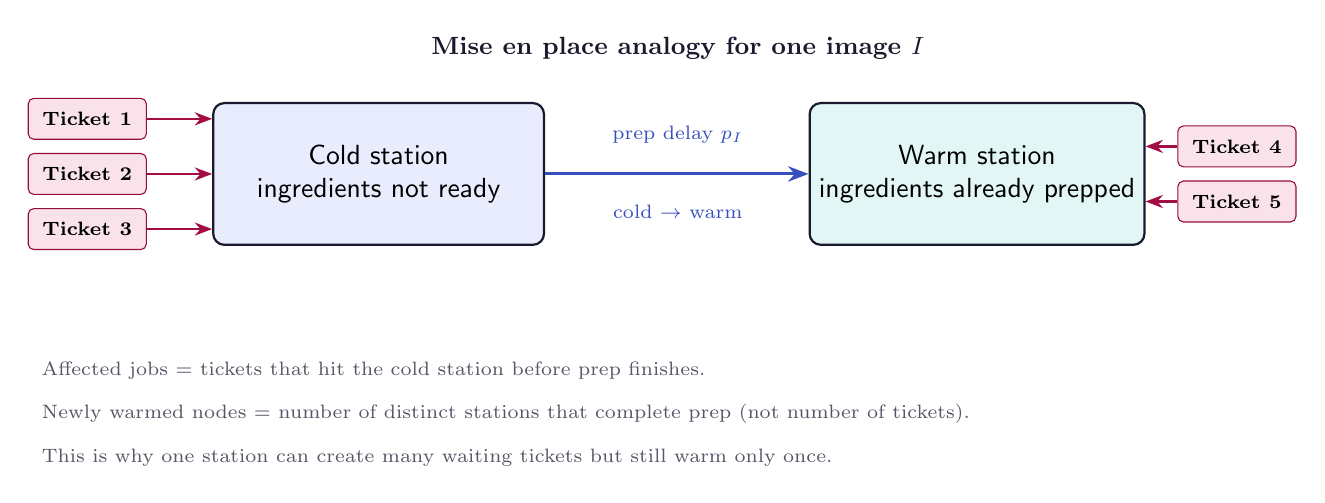
\begin{tikzpicture}[
  font=\sffamily,
  station/.style={rounded corners=4pt, draw=INK, line width=0.8pt, minimum width=4.2cm, minimum height=1.8cm, align=center},
  cold/.style={station, fill=COLD!12},
  warm/.style={station, fill=WARM!14},
  tkt/.style={rounded corners=2pt, draw=TICKET!70!black, fill=TICKET!12, minimum width=1.5cm, minimum height=0.52cm, inner sep=2pt, font=\scriptsize\bfseries},
  arr/.style={-{Stealth[length=2.2mm]}, draw=TICKET!75!black, line width=0.9pt},
  prep/.style={-{Stealth[length=2.6mm]}, draw=COLD!80!black, line width=1.1pt},
  note/.style={font=\scriptsize, text=SUB, align=left}
]

\node[font=\small\bfseries, text=INK] at (6.2, 3.5) {Mise en place analogy for one image \(I\)};

% stations
\node[cold] (s0) at (2.4, 1.9) {Cold station\\ingredients not ready};
\node[warm] (s1) at (10.0, 1.9) {Warm station\\ingredients already prepped};

% tickets toward cold station, vertically aligned with the station height
\node[tkt] (j1) at (-1.3, 2.6) {Ticket 1};
\node[tkt] (j2) at (-1.3, 1.9) {Ticket 2};
\node[tkt] (j3) at (-1.3, 1.2) {Ticket 3};
\draw[arr] (j1.east) -- (s0.west |- j1.east);
\draw[arr] (j2.east) -- (s0.west |- j2.east);
\draw[arr] (j3.east) -- (s0.west |- j3.east);

% tickets toward warm station
\node[tkt] (j4) at (13.3, 2.25) {Ticket 4};
\node[tkt] (j5) at (13.3, 1.55) {Ticket 5};
\draw[arr] (j4.west) -- (s1.east |- j4.west);
\draw[arr] (j5.west) -- (s1.east |- j5.west);

% prep transition arrow
\draw[prep] (s0.east) -- (s1.west);
\node[font=\scriptsize, text=COLD!80!black, align=center] at (6.2,2.4) {prep delay \(p_I\)};
\node[font=\scriptsize, text=COLD!80!black, align=center] at (6.2,1.42) {cold \(\rightarrow\) warm};

\node[note, anchor=west] at (-2.0, -0.6) {Affected jobs = tickets that hit the cold station before prep finishes.};
\node[note, anchor=west] at (-2.0, -1.15) {Newly warmed nodes = number of distinct stations that complete prep (not number of tickets).};
\node[note, anchor=west] at (-2.0, -1.7) {This is why one station can create many waiting tickets but still warm only once.};

\end{tikzpicture}
\end{document}
